The implementation of the breast cancer detection system was conducted in two parts. The first part corresponds to a common pipeline developed in group \citep{adam_jaamour_2020_3975093}, and the second part to individual implementations using the common pipeline as a baseline (CITE). An overview of the different pipeline parts can be found in Section~\ref{sec:implementation-detailed-flowchart}, while meeting minutes with the work distribution during the implementation of the common pipeline can be found in Appendix~\ref{ch:appendix-team-meeting-summaries}.

%%%%%%%%%%%%%%%%%%%%%%%%%%%%%%%%%%%%%%%%%%%%%
%%%%%%%%%%%%%%%%%%%%%%%%%%%%%%%%%%%%%%%%%%%%%
%%%%%%%%%%%%%%%%%%%%%%%%%%%%%%%%%%%%%%%%%%%%%

\section{Code Design}

The code, all stored in the \textit{src} directory is designed by splitting essential code into functions spread across multiple python modules, which are all organised into different directories based on the kind of task they are designed to carry out (see Appendix~\ref{ch:appendix-coding-project-structure}).\\

\textbf{Flow of execution} \space The program entry point is in the ``main.py'' module, which parses command-line arguments used to execute different parts of the program (e.g. which dataset to use) and stores them in ``config.py''. The main flow of the pipeline is controlled in ``main.py'', enclosing calls to different functions for processing the data, creating the CNN models and evaluating the results based on the CLI arguments selected.\\

\textbf{Data pre-processing} \space Functions linked to data pre-processing, such as retrieving image paths and labels, processing images, encoding labels, loading the data into memory and applying transformations for data augmentation, are all located in the \textit{data\_operations} directory. The single-run scripts for initially parsing the images' paths and labels for each dataset are in the \textit{dataset\_processing\_scripts} directory.\\

\textbf{CNN Model} \space All CNN-related code, from creating the Keras model to compiling it, fitting it, making predictions or evaluating it is placed in a custom \textit{CNN\_Model} class, which can be found in the \textit{cnn\_models.py} module. Each model is then placed in individual modules in the \textit{cnn\_models} directory.\\

\textbf{Results visualisation} \space Functions handling result visualisations in the form of plots and CSV reports are all situated in the \textit{data\_visualisation} directory. Each figure and CSV report is saved in an \textit{output} directory, while model weights are stored on an external filesystem (BigTMP) due to their large size.\\

\textbf{Other} \space General functions for printing information in the terminal and common operations are all located in the \textit{utils.py} module, while global command-line arguments used throughout the code are all stored in the \textit{config.py} module.

%%%%%%%%%%%%%%%%%%%%%%%%%%%%%%%%%%%%%%%%%%%%%
%%%%%%%%%%%%%%%%%%%%%%%%%%%%%%%%%%%%%%%%%%%%%
%%%%%%%%%%%%%%%%%%%%%%%%%%%%%%%%%%%%%%%%%%%%%

\section{General}

\subsection{Command-Line Interface}

Python's \textit{argparse} module is used to implement the CLI application, accepting different arguments (e.g. dataset,  type of mammogram, CNN base model, learning rate, batch size, maximum number of epochs, etc.) that are used across the pipeline to execute different sections of the code or use different hyperparameters (see Appendix~\ref{sec:appendix-individual-pipeline-instructions}). The values passed through the command-line are then stored as variables in the \textit{config.py} module.

\subsection{Results reproducibility}
\label{sec:implementation-results-reproducibility}

To reproduce results across different runs, random number generators are seeded with an identical value set to \textit{$111$}. The NumPy seed and Tensorflow seeds are both set to \textit{$111$}, as well as functions that include randomness such as the dataset splits to ensure that constant shuffle indices are used (Scikit-Learn's \textit{train\_test\_split}) and the dropout layer to ensure that the same random neurons are dropped:

\begin{lstlisting}[numbers=none]
# Random number generators.
numpy.random.seed(config.RANDOM_SEED)  # NumPy
tf.random.set_seed(config.RANDOM_SEED)  # Tensorflow

# Dataset splits.
_, _, _, _ = train_test_split(dataset, labels, test_size=0.25, stratify=labels, random_state=config.RANDOM_SEED, shuffle=True)

# Dropout layer.
fully_connected.add(Dropout(0.2, seed=config.RANDOM_SEED))
\end{lstlisting}

%%%%%%%%%%%%%%%%%%%%%%%%%%%%%%%%%%%%%%%%%%%%%
%%%%%%%%%%%%%%%%%%%%%%%%%%%%%%%%%%%%%%%%%%%%%
%%%%%%%%%%%%%%%%%%%%%%%%%%%%%%%%%%%%%%%%%%%%%

\section{Data Pre-Processing}

\subsection{Initial Dataset Processing}

When downloaded, both datasets contain nested directories with the mammogram images and CSV files mapping images to their label, along with additional information, e.g. breast densities, left or right breast, mass shape, etc. Two distinct Python scripts are written to parse these CSV files.\\

\textbf{mini-MIAS} \space The data is first cleaned by replacing empty cells with the ``N'' character for normal cases (only benign and malignant cases are specified initially), and each image is converted from PGM to PNG format before being saved in labelled directories rather than one vast directory.\\

\textbf{CBIS-DDSM} \space Mass and calcification mammograms are grouped into the same set by creating a new CSV file for training and testing data containing the image name, its path and its label. The CBIS-DDSM dataset is not stored locally as its size exceeds 160GB, and is therefore stored on \textit{BigTMP}, a 15TB filesystem that is mounted on the Centos 7 computer lab clients.

%%%%%%%%%%%

\subsection{Data Loading}

The data is loaded by parsing the generated CSV files mentioned above, loading mammograms and their labels simultaneously. In the case of the CBIS-DDSM dataset, a Tensorflow \textit{Dataset} is used to handle its large size by loading consecutive images into batches and caching the loaded data. This process is optimised by importing the data with parallel optimisations through Keras' \textit{prefetch method} and the \textit{data.experimental.AUTOTUNE} option. No loading optimisations are used for the smaller mini-MIAS dataset.\\

%%%%%%%%%%%

\subsection{Data Processing}

\paragraph{Image processing} 

The mini-MIAS mammograms are first imported through Keras' \textit{load\_img} function in Python Imaging Library (PIL) format and resized to a target size in pixels (e.g. 224 x 224 pixels) in greyscale (single channel) before being converted to array format using the \textit{img\_to\_array} function to be compatible with the Keras CNN models expected input. Additionally, if the \textit{roi} flag is \textit{True}, then the images are cropped around a 224 x 224 ROI (Region of Interest) in the presence of an abnormality; otherwise around a 224 x 224 region in the centre of the image.\\

The images are then normalised by dividing their pixel intensities by 255 to fit in the range of floats between 0 and 1. Because the CBIS-DDSM mammograms being in DICOM format, they first need to be imported as raw bytes before being decoded using Tensorflow I/O's \textit{decode\_dicom\_image} function. The image is then converted to PNG before following the same process as the mini-MIAS images.

\paragraph{Label encoding}

In the case of multi-class classification, Scikit-Learn's \textit{LabelEncoder} class is used to one-hot encode labels, whereas Keras' \textit{to\_categorical} function is used to convert labels to a binary class matrix in the case of binary classification.

%%%%%%%%%%%

\subsection{Dataset Splits}

Scikit-Learn's \textit{train\_test\_split} function is used to split the dataset into a training, validation and testing set (see Figure~\ref{fig:dataset_splits}). A 60/20/20\% shuffled stratified split is conducted to maintain class balance across the sets and avoid data bias when training the model. 

\begin{figure}[ht]
\centerline{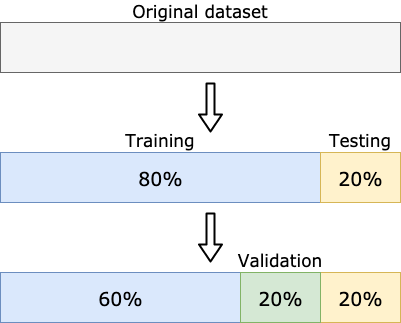
\includegraphics[width=0.55\textwidth]{figures/implementation/dataset_splits.png}}
\caption{\label{fig:dataset_splits}Original dataset divided into training, validation and testing sets using a 60/20/20\% split.}
\end{figure}

%%%%%%%%%%%

\subsection{Data Augmentation \& Class Balance}

For the highly imbalanced mini-MIAS dataset, image augmentation is used to balance the class distribution. Random amounts of rotations and shears between -20 and 20 degrees, noise and horizontal flips are added to existing images of the minority classes to balance the dataset. The transformations are all achieved through the Scikit-Image library. These are then shuffled to ensure that newly generated images are not grouped together. An example of the possible transformations is shown in Figure~\ref{fig:implementation-Data augmentation transforms}.\\

\begin{figure}[h]
\centerline{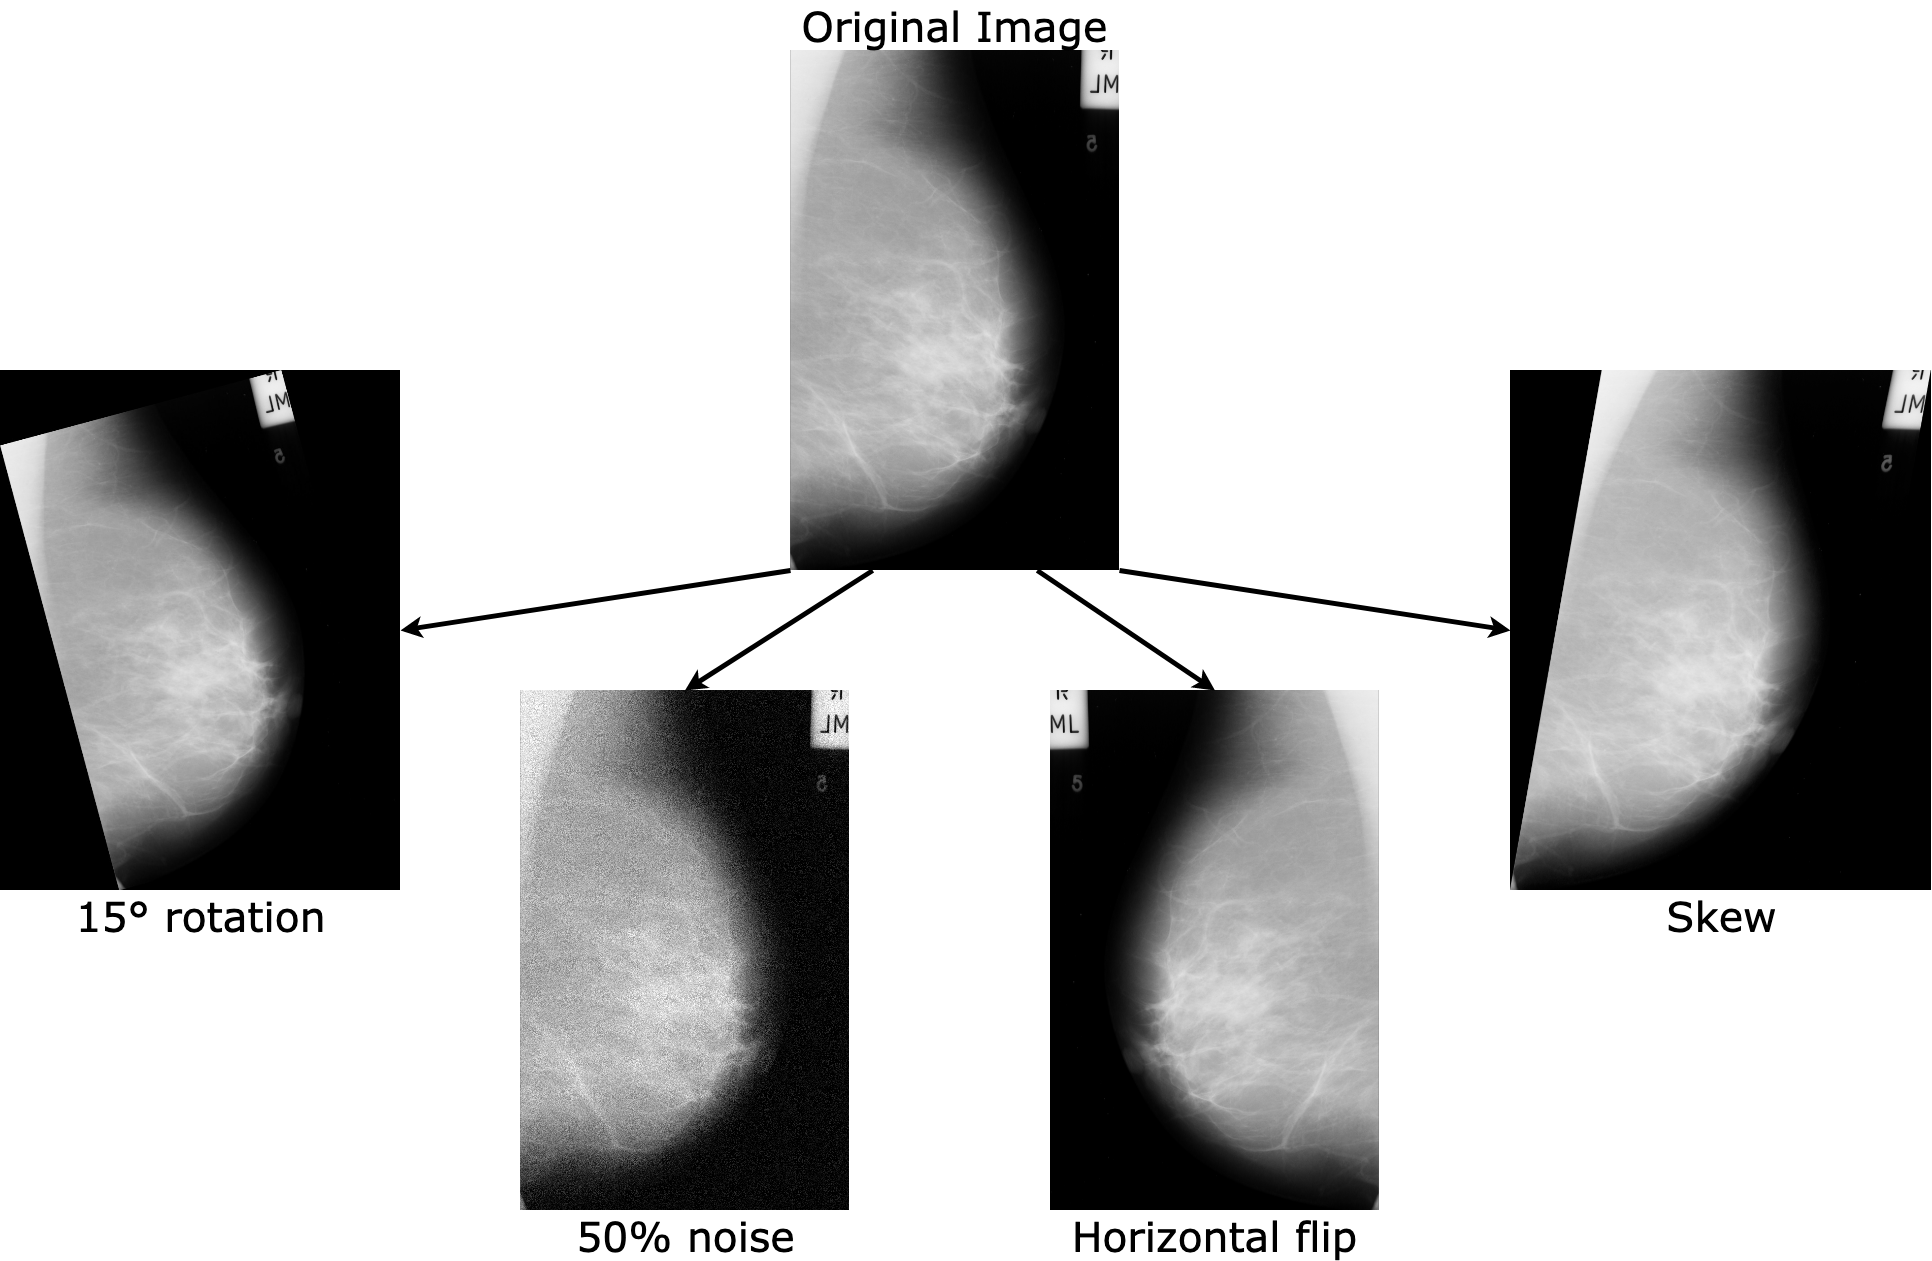
\includegraphics[width=\textwidth]{figures/implementation/Data augmentation transforms.png}}
\caption{\label{fig:implementation-Data augmentation transforms}Example of affine transforms applied to mini-MIAS mammograms to generate new samples. Original image retrieved from the mini-MIAS dataset \citep{Suckling1994}.}
\end{figure}

A computationally-cheaper alternative consists of calculating class weights to balance the classes, giving larger weights to the minority class and smaller weights to the majority class. For example, in the case of the CBIS-DDSM dataset (see Section~\ref{sec:design-dataset-balance}), a weight of 0.907 can be used for benign samples and 1.113 for malignant samples to balance the dataset. These weights are calculated by using Scikit-Learn's \textit{compute\_class\_weights} function with the ``balanced'' argument.

%%%%%%%%%%%%%%%%%%%%%%%%%%%%%%%%%%%%%%%%%%%%%
%%%%%%%%%%%%%%%%%%%%%%%%%%%%%%%%%%%%%%%%%%%%%
%%%%%%%%%%%%%%%%%%%%%%%%%%%%%%%%%%%%%%%%%%%%%

\section{Model Training}

\subsection{Sequential Model}
\label{sec:implementation-sequential-cnn-model}

The CNN model is created in Keras through the custom \textit{Cnn\_model} class. The Keras \textit{Sequential} class is used to create the CNN model described in Section~\ref{sec:design-cnn-model-decision} by linearly stacking layers on top of one another. The input layer size is first specified to match the target size chosen in the pre-processing steps. Because a CNN pre-trained on ImageNet with RGB images (three channels) is used, the greyscale images have to be concatenated into a triple channel greyscale input:

\begin{lstlisting}[numbers=none]
img_input = Input(shape=(config.IMG_SIZE['HEIGHT'], config.IMG_SIZE['WIDTH'], 1))
img_conc = Concatenate()([img_input, img_input, img_input])
\end{lstlisting}

Next, the CNN architecture pre-trained on ImageNet is used through the Keras Application API, allowing any CNN to be used such as VGG19 or MobileNetV2. The fully connected layers are dropped by adding \textit{include\_top=False} to the imported model. To download the ImageNet weights automatically, the following line of code is included to bypass SSL certificate verifications:

\begin{lstlisting}[numbers=none]
ssl._create_default_https_context = ssl._create_unverified_context
model_base = MobileNetV2(include_top=False, weights="imagenet", input_tensor=img_conc)
\end{lstlisting}

Next, a \textit{Flatten} layer is added to convert the data from 2D to 1D, making it compatible with a fully-connected MLP. In this MLP, a dropout layer with a rate of 0.2 is added, followed by two dense hidden layers (one with 512 neurons, the other with 32 neurons). Finally, the output layer is appended at the end of the sequential model, with either a sigmoid activation function if the CBIS-DDSM dataset is used or a softmax activation function if the mini-MIAS dataset is used.

TODO: ADD SUMMARY PIC

% Additional convolution and pooling layers are added before the pre-trained model to accommodate larger images. These are slowly reduced in size as they go through the pooling layers, allowing lower-level features to be learned before passing through the VGG19 model.\\

% Image sizes of 1024x1024px large used and downscaled using convolutional layers. This size was chosen as it is the size of the mini-MIAS dataset images, which will be used to initially train the CNN before training on the large CBIS-DDSM dataset.\\

\subsection{Training Steps} 

The training phase is separated in two steps, as mentioned in Section~\ref{sec:design-transfer-learning-training-phase}. To freeze the pre-trained base model's layers, the \textit{trainable} attribute is set to \textit{False}, allowing only the MLP's fully connected layers to learn (weights are not updated). During this step, the learning rate and the maximum number of epochs are set by the CLI arguments, which default to $0.001$ and $150$ respectively. Once training converges, all layers are unfrozen by setting \textit{trainable} attribute to \textit{True} and a second training phase is launched with a lower learning rate set to $0.00001$.\\

Tensorflow \textit{Callbacks} are used to enable early stopping conditions, which are set to halt training when the validation loss does not improve after the maximum number epochs specified divided by 10 (e.g. $150/10=15$). Additionally, an option to reduce the learning rate on plateaus is used to avoid increasing the validation loss when the learning stagnates, which is set at half the previously mentioned patience.\\

For the CBIS-DDSM dataset, the \textit{BinaryCrossentropy} loss and \textit{BinaryAccuracy} are used, whereas \textit{CategoricalCrossentropy} and \textit{CategoricalAccuracy} are used for the mini-MIAS dataset. This is necessary as different forms of cross entropy and accuracy equations have to be used to accommodate the binary classification tasks which have labels encoded differently (binary-encoded labels for CBIS-DDSM and one-hot-encoded labels for mini-MIAS).

\subsection{Model \& Weights Saving}
\label{sec:implementation-model-saving-minimiasbinary}

Once the CNN is finished training, the full model, including the model's configuration, the layer hyperparameters, the optimiser, the training results (losses and metrics), and the model's state (layer weights) are saved in HDF5 format (``.h5'' file extension) to be re-used in the future, especially for the model's final evaluation on the test set. Additionally, specific layer weights are saved for transfer learning experiments, such as the entire model's weights or the fully connected layers' weights only, to test different levels of transfer learning (see Section~\ref{sec:evaluation-transfer-learning}).\\

To perform transfer learning from the mini-MIAS dataset to the CBIS-DDSM dataset, the mini-MIAS dataset is binarised by dropping normal cases altogether, creating a tiny dataset of 115 abnormal images (64 benign and 51 malignant). The model is then trained on the binary mini-MIAS dataset and its final weights are saved in NumPy format. These weights can be loaded when instantiating a new model for fitting the CBIS-DDSM dataset.

%%%%%%%%%%%%%%%%%%%%%%%%%%%%%%%%%%%%%%%%%%%%%

\section{Predictions \& Results visualisation}

Once the model is trained, predictions can be made through the \textit{make\_prediction} function by passing in new images and their ground truth labels. These predictions are then evaluated through the metrics mentioned in Section~\ref{sec:design-results-visualisation}. The accuracy, precision, recall, F1 score and confusion matrices are all calculated via Scikit-Learn's \textit{metrics} API. Additionally, the evolution of the loss and accuracy on the training and validation sets are all plotted against the number of epochs during both phases of training to assess how well the model learned the data and where improvements could be made. The results above are either saved in CSV files or plotted using Matplotlib and Seaborn before being saved in PNG format to later be referenced in Chapter~\ref{ch:chapter-evaluation}.\\

During the development of this pipeline, the validation set was used to assess the performance of the model without snooping into the test dataset, which was reserved for the final evaluation of the model in Chapter~\ref{ch:chapter-evaluation}.

%%%%%%%%%%%%%%%%%%%%%%%%%%%%%%%%%%%%%%%%%%%%%
%%%%%%%%%%%%%%%%%%%%%%%%%%%%%%%%%%%%%%%%%%%%%
%%%%%%%%%%%%%%%%%%%%%%%%%%%%%%%%%%%%%%%%%%%%%

\section{Pipeline Flowchart}
\label{sec:implementation-detailed-flowchart}

The flowchart in Figure~\ref{fig:implementation-flowchart} reveals which sections of the pipeline were implemented as a group, later amended, and implemented individually.

\begin{figure}[h]
\centerline{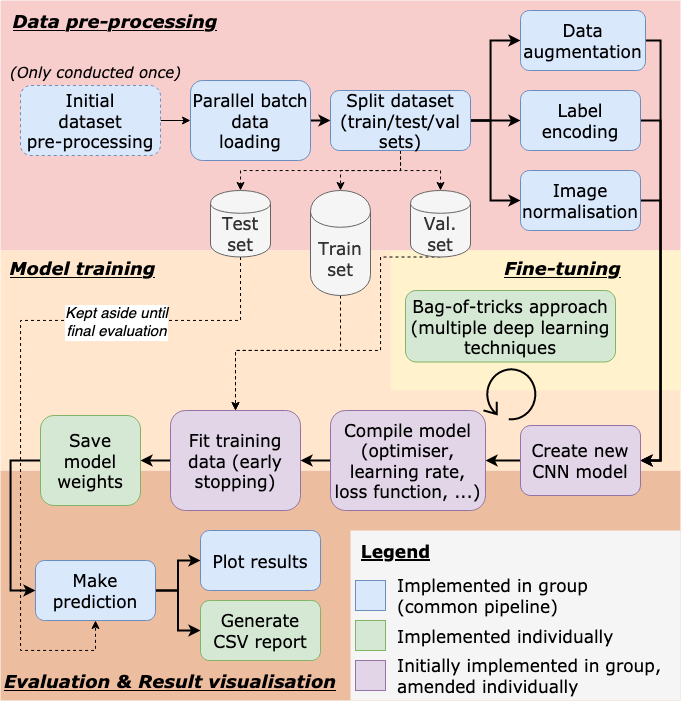
\includegraphics[width=\textwidth]{figures/implementation/implementation flowchart.png}}
\caption{\label{fig:implementation-flowchart}A detailed flowchart of the breast cancer detection deep learning pipeline implemented, separated between data pre-processing, model training, results visualisation and fine-tuning.}
\end{figure}
